\partabstractfp{\textbf{This is the abstract of this part}. \lipsum[10]}
\partabstractrp{\lipsum[11]}
\partabstractlettrine{A}{bstract} % the first word of the abstract

\part{QUESTIONS}

\chapter{Tables and figures}
\section{(title section 1)}
\subsection{(title sub-section 1)}

\lipsum[1]

\textbf{Here is an example of a wide table.}
%\begin{widetable}[!htbp]
\begin{table*}[!htbp]
\setmathfont[Path = fonts/]{Geometric415BT-Lite.ttf}
\ttabbox
{\caption{Balance sheet U.S. households, 2006}}
{
\begin{tabular*}{\caplength}{@{\extracolsep{\fill}}@{\hspace{1em}}lr.lr.}
    \hspace{-1em}\textbf{Assets}              &\textbf{\$ Billion}     &\hed{\textbf{\% Total}}   &\textbf{\makecell[lb]{Liabilities\\and Net Worth}}   &\textbf{\$ Billion}     &\hed{\textbf{\% Total}}\\
    \addlinespace
    Real assets\\
    Real estate         &\$22,177       &33.6\%           &Mortgages          &\$9,161  &13.9\%\\
    Consumer durables   &3,822          &5.8              &Consumer credit    &2,150      &3.3\\
    Other               &224            &0.3              &Bank \& other loans   &237     &0.4\\
    \addlinespace
    \cline{2-2}\cline{3-3}
    \addlinespace
    \hspace{1em}\textit{Total real assets}   &\$26,223       &39.7\%           &\hspace{1em}\textit{Total liabilities}  &\$12,199   &18.5\%\\
\end{tabular*}
\floatfoot*{Note: Column sums may differ from totals because of rounding error.\\
Source: \textit{Flow of Funds Accounts of the United States}, Board of Governors of the Federal Reserve System, June 2006.}
}
%\end{widetable}
\setmathfont[Ligatures=TeX]{xits-math.otf}
\end{table*}

\newpage
$a+c=b$, \textbf{well, equations work as normal}.

\lipsum[1]
\tmarginpar{Margin note title}{You can use margin notes like this.}
\lipsum[2]

\textbf{Here is an example of a short table.}
\begin{table}[!htbp]
\setmathfont[Path = fonts/]{Geometric415BT-Lite.ttf}
\stabbox{2.0cm}
{\caption{Domestic net worth}}
{\begin{tabular*}{\cflwidth}{@{\hspace{3pt}}@{\extracolsep{\fill}}*{8}{@{\hspace{-3pt}}c}}
    p1 & 1.7538 & -0.7698 & 1.4597 & -0.4137 & 1.2449 & -0.5518                 \\
    p2 & 1.6055 & -0.5549 & 1.2368 & 0.2507  & 1.2172 & -0.0974                 \\
    p3 & 1.5619 & 0.0799  & 1.0892 & 0.3585  & 1.2357 & -0.2726                 \\
    p4 & 1.4741 & 0.0109  & 0.9944 & 0.5935  & 1.2515 & -0.5038                 \\
\end{tabular*}
\floatfoot*{Note: Column sums may differ from totals because of rounding error. \\
Source: \textit{Flow of Funds Accounts of the United States}, Board of Governors of the Federal Reserve System, June 2006.}
}
\setmathfont[Ligatures=TeX]{xits-math.otf}
\end{table}

\lipsum[7]

\textbf{This is an example of a wide figure (odd pages).}
\begin{figure*}[!htbp]
  \wdfigbox
  {\caption{Bundling creates a complex security}}
  {
  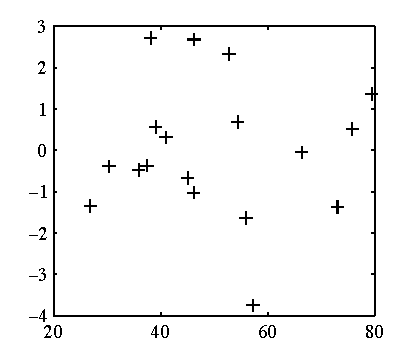
\includegraphics{./figure/sample.pdf}
  \floatfoot{Source: \textit{The Wall Street Journal}, December 19, 2001}
  }
\end{figure*}

\lipsum[7-8]

\textbf{This is an example of a wide figure (even pages).}
\begin{figure*}[!htbp]
  \wdfigbox
  {\caption{Bundling creates a complex security}}
  {
  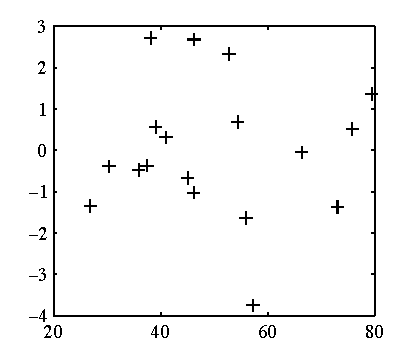
\includegraphics{./figure/sample.pdf}
  \floatfoot{Source: \textit{The Wall Street Journal}, December 19, 2001}
  }
\end{figure*}


\subsection{(title sub-section 2)}

\lipsum[1]
\tmarginpar{Margin note title}{This is a margin note, This is a margin note, This is a margin note}
\lipsum[2-5]

\section{(title section 2)}

\lipsum[1]
\tmarginpar{Margin note title}{This is a margin note, This is a margin note, This is a margin note}
\lipsum[2-5]

\subsection{(title sub-section 1)}

\lipsum[1-4]
\tmarginpar{Margin note title}{This is a margin note, This is a margin note, This is a margin note}
\lipsum[5]

\subsection{(title sub-section 2)}

\lipsum[1]
\lipsum[2-5]

\chapter{Other environments}
\section{(title section 1)}
\subsection{(title sub-section 1)}

\lipsum[9]

\textbf{This is a new example environment, you can define other similar environment in the similar way.}
\begin{example*}
  \wdexpbox
  {\caption{Bundling creates a complex security}}
  {\lipsum[10]}
\end{example*}
\newpage
\lipsum[11]

\begin{example*}
  \wdexpbox
  {\caption{Bundling creates a complex security}}
  {\lipsum[12]}
\end{example*}

\subsection{(title sub-section 2)}
\section{(title section 2)}
\subsection{(title sub-section 1)}
\subsection{(title sub-section 2)}

\partabstractfp{\lipsum[12]}
\partabstractrp{\lipsum[13]}
\partabstractlettrine{B}{bstract}

% those bunch of chapters and sections are only used for filling the table of contents :P
\part{QUESTIONS OF TECHNIQUE}
\chapter{Chapter 1}
\section{(title section 1)}
\subsection{(title sub-section 1)}
\subsection{(title sub-section 2)}
\section{(title section 2)}
\subsection{(title sub-section 1)}
\subsection{(title sub-section 2)}
\chapter{Chapter 2}
\section{(title section 1)}
\subsection{(title sub-section 1)}
\subsection{(title sub-section 2)}
\section{(title section 2)}
\subsection{(title sub-section 1)}
\subsection{(title sub-section 2)}
\chapter{Chapter 3}
\section{(title section 1)}
\subsection{(title sub-section 1)}
\subsection{(title sub-section 2)}
\section{(title section 2)}
\subsection{(title sub-section 1)}
\subsection{(title sub-section 2)}
\chapter{Chapter 4}
\section{(title section 1)}
\subsection{(title sub-section 1)}
\subsection{(title sub-section 2)}
\section{(title section 2)}
\subsection{(title sub-section 1)}
\subsection{(title sub-section 2)}
\chapter{Chapter 5}
\section{(title section 1)}
\subsection{(title sub-section 1)}
\subsection{(title sub-section 2)}
\section{(title section 2)}
\subsection{(title sub-section 1)}
\subsection{(title sub-section 2)}
\chapter{Test of large page numbers}
\section{(title section 1)}
\subsection{(title sub-section 1)}
\subsection{(title sub-section 2)}
\section{(title section 2)}
\setcounter{page}{1000}
\subsection{(title sub-section 1)}
\textbf{This is a test for large page numbers. Note that the header for titles remains the same location even if the page number is large.}

\lipsum[13-20]
\subsection{(title sub-section 2)}
\lipsum[13-20]

%%% Local Variables: 
%%% TeX-master: "book_template_2"
%%% End: 
